\documentclass[12pt, a4paper]{article}
    \usepackage[utf8]{inputenc}
    %\usepackage[english, spanish]{babel}
    %\usepackage{fullpage} % changes the margin
    \usepackage{graphicx} 
    \usepackage{enumitem} 
    \usepackage{chngcntr}
    \counterwithin{figure}{section}
    \renewcommand{\thesection}{\arabic{section}} 
    \renewcommand{\thesubsection}{\thesection.\arabic{subsection}}
    \renewcommand{\baselinestretch}{1.5}

    \usepackage{amsmath}
    \usepackage{mathptmx}
    \usepackage[spanish, es-tabla]{babel}
    \usepackage{amssymb}
    \usepackage{makeidx}
    \usepackage{float}
    \pagenumbering{arabic}
    \usepackage[left=25mm, right=25mm, top=25mm, bottom=25mm]{geometry}

    \usepackage[backend=biber]{biblatex}
    \bibliography{referencias}

\begin{document}

    \begin{titlepage}
        \centering
        {\scshape\Large Universidad Central de Venezuela \par}
        {\scshape\Large Facultad de ingeniería \par}
        {\scshape\Large Escuela de ingeniería Eléctrica \par}
        {\scshape\Large Departamento de Electrónica, Computación y Control \par}

        \vspace{6cm}
        {\Large\bfseries LABORATORIO-6 : Amplificador JFET\par}
        \vspace{6cm}

        \vfill
        %\begin{flushleft}
        %    Auxiliar docente:\par
        %    Tovar José
        %\end{flushleft}
        %\vspace{-2cm} %pendiente
        \begin{flushright}
            Estudiantes:\par
            Santana Ricardo C.I.:29571461 \par
            Fajardo Carla C.I.:27571576
            \vspace{1cm}  
        \end{flushright}
        \vfill
        {\large 1 marzo 2024 \par}
    \end{titlepage}

    \tableofcontents

    \newpage

    \section{Resumen}

    La práctica de laboratorio a presentar consistió en estudiar el funcionamiento dinámico para pequeña señalde un amplificador JFET canal n. Se obtuvo su punto estático de operación además se tomaron mediciones de las señales de entrada y de salida del amplificador para luego obtener la impedancia de entrada, la impedancia de salida así como también la ganancia de tensión. Se hace la observación que para esta práctica no se consiguió la resistencia de 6,2kΩ, por lo que se utilizaron dos resistencias en serie, una de 2.7k \Omega y otra de 3.6k \Omega, por lo que se puede decir que se utilizó una resistencia equivalente de 6.3k \Omega .
    
    \newpage

    \section{Introducción}

    Existen diversos tipos de transistores con distintas aplicaciones. Entre ellos, cabe destacar el transistor de efecto de campo (FET), el cual controla la corriente que circula por uno de sus pines a través del voltaje aplicado entre sus otros dos terminales.
    
    Comprender el funcionamiento de este dispositivo tanto estática como dinamicamente es de suma importancia, ya que su uso permite obtener ganancias de señal elevadas y una alta impedancia de entrada. Estas características resultan fundamentales en la amplificación de señales débiles y en la reducción de ruido en circuitos electrónicos. Los amplificadores JFET tienen variadas aplicaciones y se utilizan en diferentes áreas. Por ejemplo, son empleados en sistemas de audio de alta calidad, en instrumentos de medición y control de procesos industriales, así como en sistemas de comunicación inalámbrica, entre otros.

    En el siguiente prelaboratorio, se investigará el diseño y la implementación de un amplificador que utiliza un JFET, además se analizará los efectos sobre el punto de operación de la variación de su resistencia de drenaje mediante el uso de un potenciómetro. 

    \newpage

    \section{Objetivos}
    
    \subsection{Objetivo General}
    \begin{itemize}
        \item Analizar el funcionamiento de un transistor JFET como amplificador.
    \end{itemize}

    \subsection{Objetivos Específicos}
    \begin{itemize}
        \item Estudiar el comportamiento dinámico de una estructura básica amplificadora JFET canal n.
        \item Obtener experimentalmente las características más importantes de un amplificador como son: la ganancia de tensión, impedancia de entrada e impedancia de salida.
    \end{itemize}

    \newpage

    \section{Marco Teórico}

    \subsection{Modelo de pequeña señal para transistores FET [1]}

    El circuito equivalente de pequeña señal de un transistor FET se puede obtener por métodos análogos a los utilizados en transistores bipolares. Sin embargo, al ser dispositivos controlados por tensión, el modelo bipuerta más adecuado es el de parámetros $\{Y\}$, ya que relacionan las corrientes de salida con tensiones de entrada. La figura \ref{fig:mt1} representa el modelo de pequeña señal de un FET constituido por dos parámetros: $g_m$, o factor de admitancia, y $r_d$, o resistencia de salida o resistencia de drenador. Esta notación es la más extendida para describir estos parámetros, aunque algunos fabricantes utilizan la notación en parámetros $\{Y\}$ o $\{G\}$, denominando $y_{fs}$ o $g_{fs}$ a $g_m$, e $y_{os}^{-1}$ o $g_{os}^{-1}$ o $r_oss$ a $r_d$. Estos parámetros dependen de la corriente de polarización del transistor (ID), y el fabricante proporciona las curvas que permiten extraer sus valores en diferentes condiciones de polarización. A continuación se describe con más detalle los parámetros $g_m$ y $r_d$.

    \begin{figure}[h!]
        \centering
        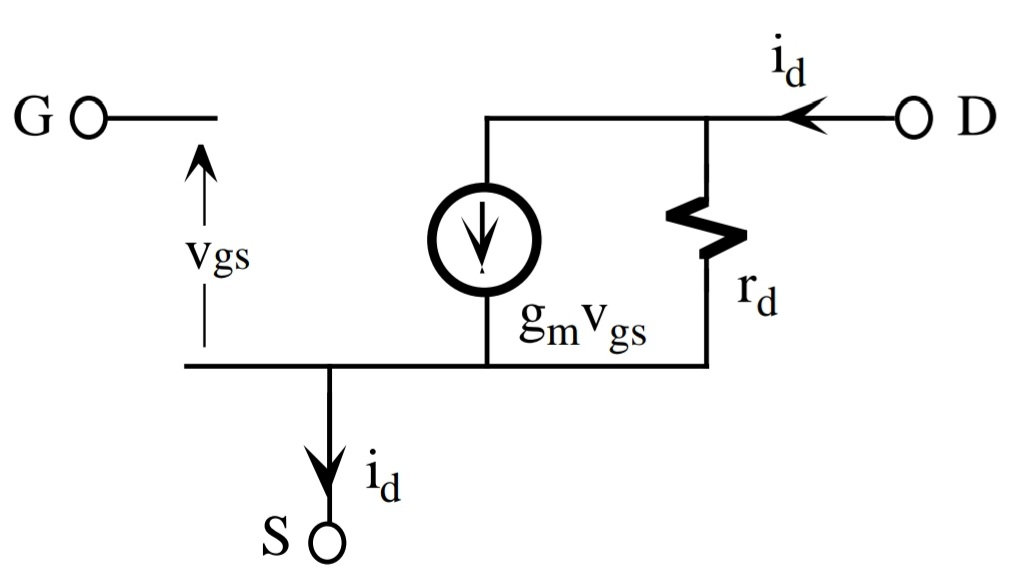
\includegraphics[height=5cm\textwidth]{pequenasenal.jpg}
        \caption{Modelo de pequeña señal de un transistor FET.}
        \label{fig:mt1}
    \end{figure}

    {\bf Factor de admitancia gm.} Se define este parámetro como

    \begin{equation} \label{eqgm}
        g_m = \left.\frac{\Delta I_D}{\Delta V_{GS}}\right|_{V_{DSQ}} = \left.\frac{I_{D2}-I_{D1}}{V_{GS2}-V_{GS1}}\right|_{V_{DSQ}} = \left.\frac{\Delta i_d}{\Delta v_{gs}}\right|_{V_{DSQ}}
    \end{equation}

    En un JFET, $g_m$ se puede extraer a partir de la ecuación analítica del transistor en la región de saturación que relaciona la $I_D$ con la $V_GS$, definida por

    \begin{equation} \label{eqvgs}
        I_D = I_{DSS}\left(1-\frac{V_{GS}}{V_P}\right)^2 \;\;\; ó \;\;\; 1-\frac{V_{GS}}{V_P} = \sqrt{\frac{I_D}{I_{DSS}}}
    \end{equation}

    En la ecuación \eqref{eqgm}, $g_m$ es un parámetro definido por cociente de incrementos que se pueden aproximar por derivadas, de forma que aplicando esta definición a la ecuación \eqref{eqvgs} y resolviendo se obtiene que

    \begin{equation} \label{eqdgm}
        g_m = \left.\frac{d I_D}{d V_{GS}}\right|_{V_{DSQ}} = -\frac{2I_{DSS}}{V_P}\left(1-\frac{V_{GS}}{V_P}\right) = -\frac{2}{V_P}\sqrt{I_DI_{DSS}}
    \end{equation}

    {\bf Resistencia de salida o de drenador rd.} Se define como

    \begin{equation} \label{eqrd}
        r_d = \left.\frac{\Delta V_{DS}}{\Delta I_D}\right|_{V_{GSQ}} = \left.\frac{V_{DS2}-V_{DS1}}{I_{D2}-I_{D1}}\right|_{V_{GSQ}} = \left.\frac{\Delta v_{ds}}{\Delta i_d}\right|_{V_{GSQ}}
    \end{equation}

    Factor de amplificación $\mu$. Relaciona los parámetros $g_m$ y $r_d$ de la siguiente manera

    \begin{equation} \label{eqmu}
        \mu = \frac{\Delta V_{DS}}{\Delta V_{GS}} = \frac{\Delta I_D}{\Delta V_{GS}}\frac{\Delta V_{DS}}{\Delta I_D} = g_mr_d
    \end{equation}

    Las definiciones gráficas de $g_m$ y $r_d$ se encuentran en las figuras \ref{fig:mt2} y \ref{fig:mt3}.

    \begin{figure}[h!]
        \centering
        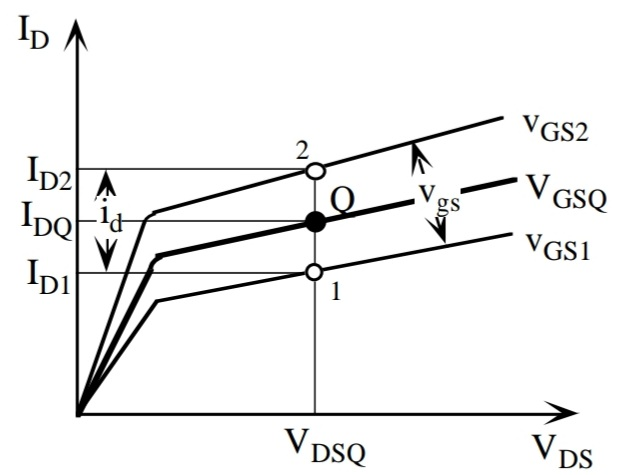
\includegraphics[height=5cm\textwidth]{grafgm.jpg}
        \caption{Definición gráfica de $g_m$.}
        \label{fig:mt2}
    \end{figure}

    \begin{figure}[h!]
        \centering
        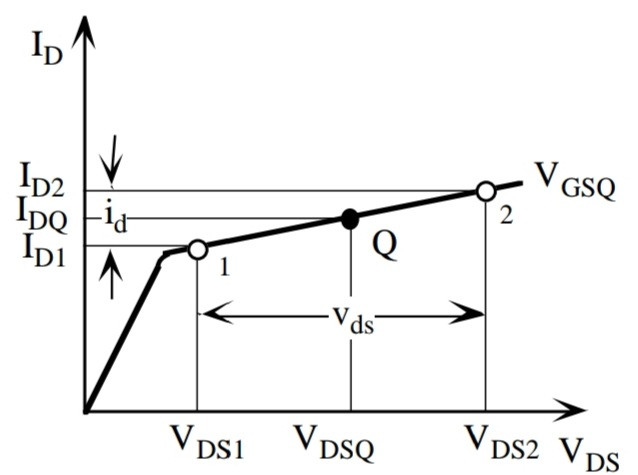
\includegraphics[height=5cm\textwidth]{grafrd.jpg}
        \caption{Definición gráfica de $r_d$.}
        \label{fig:mt3}
    \end{figure}

    En la \ref{tab:mt1} se resume los configuraciones más utilizadas de amplificadores básicos basados en transistores FET, bien sea JFET o MOSFET. Estas configuraciones son: fuente común, fuente común con resistencia de fuente, puerta-común y drenador común. Las ecuaciones indicadas en la derecha permite obtener el modelo equivalente en tensión de los diferentes circuitos. Un FET operando en fuente común presenta la mayor ganancia en tensión aunque ésta sea muy inferior a los valores de E-C en transistores bipolares. La configuración drenador común tiene una ganancia ligeramente inferior a 1, similar al C-C en transistores bipolares.

    \begin{table}[h!]
        \centering
        \caption{Análisis de las configuraciones básicas de los amplificadores JFET y MOSFET.} 
        \label{tab:mt1}
        \begin{tabular}{c}
            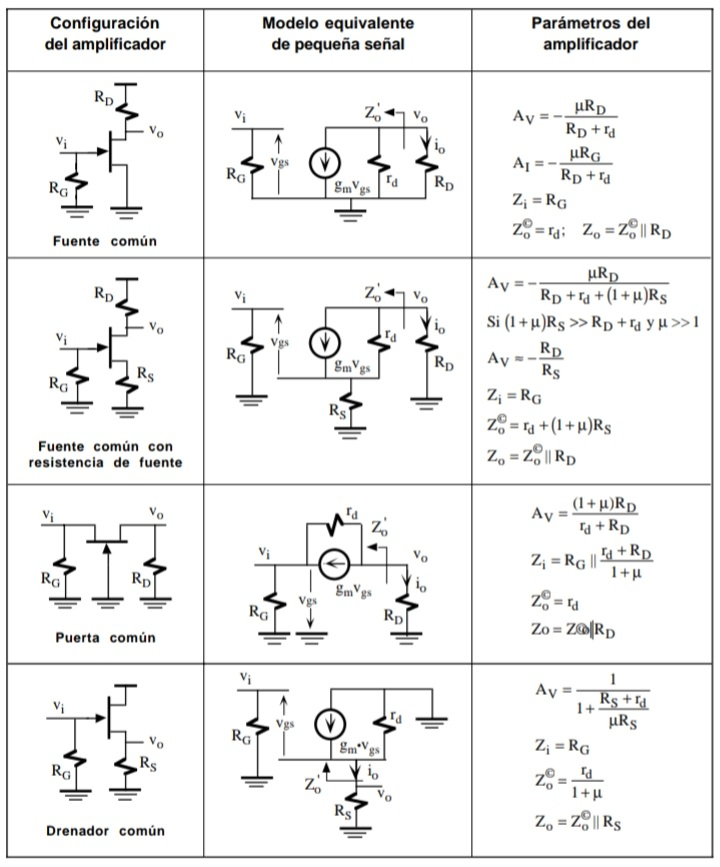
\includegraphics[width=16cm\textwidth]{configuraciones.jpg} \\
        \end{tabular}
    \end{table}

    \newpage

    \section{Metodología}

    \subsection{Trabajo Previo al Laboratorio}

    Para el circuito de la Figura \ref{fig:amp}:

    \begin{figure}[h!]
        \centering
        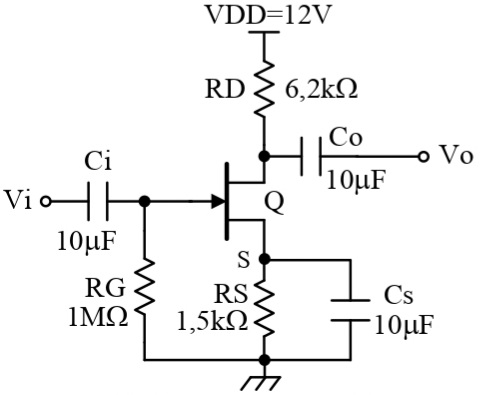
\includegraphics[height=5cm\textwidth]{amplificador.jpg}
        \caption{Amplificador JFET}
        \label{fig:amp}
    \end{figure}

    Se calculó:

    \begin{enumerate}
        \item \label{p11}	Punto estático de operación $(I_{DQ}, V_{DSQ})$.
        \item \label{p12}	La ganancia de tensión Av, Impedancia de entrada Zin e Impedancia de salida Zout.
    \end{enumerate}

    \subsection{Trabajo de Laboratorio}

    \begin{enumerate}
        \item \label{p21}   Se midió el punto estático de operación.
        \item \label{p22}	Se colocó en el generador una señal senoidal de frecuencia 1kHz, promedio nulo y amplitud 1Vp-p.
        \item \label{p23} 	Se observó, con el osciloscopio en doble canal, las formas de onda de la entrada Vi y la salida Vo. Se tomó captura de ambas formas de onda para luego en el informe, en el punto del análisis de resultados, se compare en cuanto a su forma, frecuencia y amplitud. Se midió la tensión de entrada y de salida pico-pico.
        \item \label{p24} 	Se subió la amplitud de la señal de entrada hasta el punto donde comienza a distorsionarse la señal de salida. Se midió la amplitud pico-pico de la señal de entrada. Se tomó captura de ambas formas de onda.
        \item \label{p25} 	Se subió hasta el máximo la amplitud de la señal de entrada y se midió esta amplitud pico-pico. Se tomó captura de las ondas de entrada y salida.
        \item \label{p26} Se midió experimentalmente los valores de tensiones para luego determinar en el informe las impedancias de entrada y de salida del amplificador.
    \end{enumerate}

    \newpage

    \section{Cálculos prévios}

    Se trabajará con el transistor FET canal n 2N5555, el cual posee las siguientes especificaciones:
    
    \begin{table}[h!]
        \centering
        \caption{Características del transistor 2N5555} %nombre de la tabla
        \label{tab:5555} %indice de la tabla
        \begin{tabular}{c}
            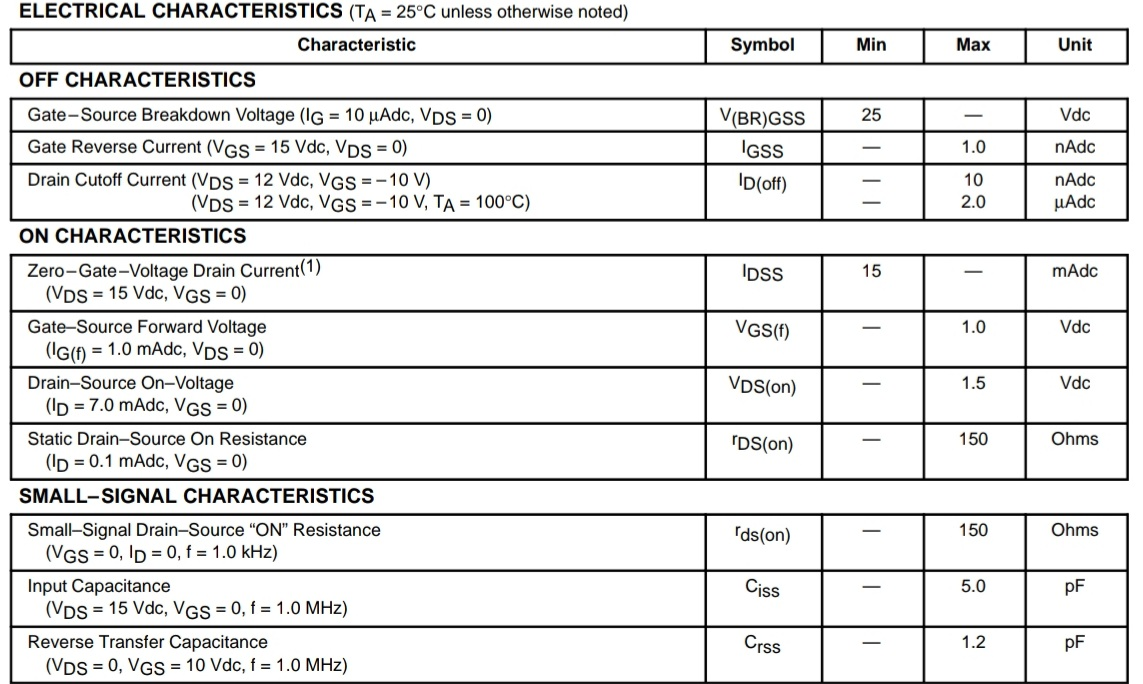
\includegraphics[width=16cm\textwidth]{2N5555.jpg} \\
        \end{tabular}
    \end{table}
    
    de las cuales se deduce por promediación que:

    $V_P = -1V$

    $I_{DSS} = 15mA$

    Entonces analizando el circuito de la figura \ref{fig:cir1}, para encontrar el punto estático de operación $Q(V_{DSQ},I_{DQ})$, donde los condensadores se desacoplan por estar trabajando en DC.

    \begin{figure}[h!]
        \centering
        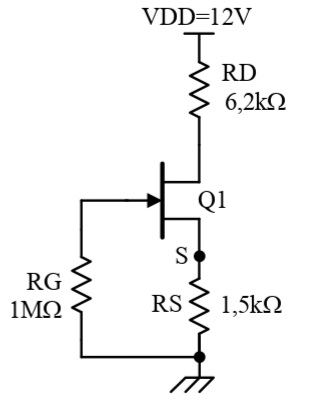
\includegraphics[height=5cm\textwidth]{circuito1.jpg}
        \caption{Polarización del JFET canal n.}
        \label{fig:cir1}
    \end{figure}

    Se tiene un JFET autopolarizado. Esto es debido a que la corriente circulando por $R_G$ es cero y, por tanto, toda la corriente ($I_D$) que entra por el drenador D sale por la fuente S.

    Analizando la malla relacionada al circuito de la compuerta con $I_G = 0$,

    $$V_{GS} = -I_DR_S \rightarrow I_D = -{V_{GS} \over R_S}$$

    \begin{equation} \label{eq1}
        I_D = -{V_{GS} \over R_S}
    \end{equation}

    Conociendo la características de transferencia de un JFET que relaciona $V_{GS}$ e $I_D$ por la fórmula \eqref{eqvgs}

    \begin{equation*}
        I_D = I_{DSS}\left( 1-{V_{GS} \over V_P}\right) ^2
    \end{equation*}

    Entonces

    $$I_{DQ} = I_{DSS}\left( 1-{V_{GSQ} \over V_P}\right) ^2 = -{V_{GSQ} \over R_S}$$

    buscando $V_{GSQ}$
    
    \begin{equation}
        \label{eq3}
        \begin{split}
            I_{DSS}\left( 1-{V_{GSQ} \over V_P}\right) ^2  & = -{V_{GSQ} \over R_S} \\
            1 - 2{V_{GSQ} \over V_P} + ({V_{GSQ} \over V_P})^2  & = -{V_{GSQ} \over I_{DSS}R_S} \\
            1 - 2{V_{GSQ} \over V_P} + {V_{GSQ}^2 \over V_P^2} + {V_{GSQ} \over I_{DSS}R_S} & = 0 \\
            {1 \over V_P^2}V_{GSQ}^2 + \left({1 \over I_{DSS}R_S} - {2 \over V_P}\right)V_{GSQ} + 1 & = 0 \\
        \end{split}
    \end{equation}

    Reemplazando valores conocidos en \eqref{eq3} y resolviendo ecuación de segundo grado

    \begin{split}
        {1 \over V_P^2}V_{GSQ}^2 + \left({1 \over I_{DSS}R_S} - {2 \over V_P}\right)V_{GSQ} + 1 & = 0 \\
        {1 \over (-1V)^2}V_{GSQ}^2 + \left({1 \over (15mA)(1.5k\Omega)} - {2 \over (-1V)}\right)V_{GSQ} + 1 & = 0 \\
        V_{GSQ}^2 + {92 \over 45}V_{GSQ} + 1 & = 0 \\
    \end{split}

    $$V_{GSQ} = -0.81V$$

    \begin{figure}[h!]
        \centering
        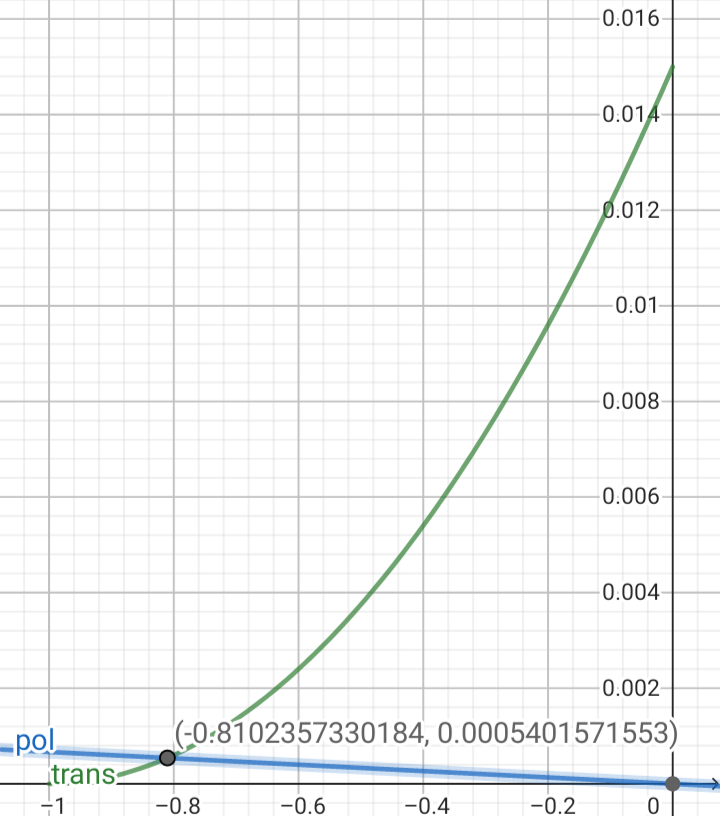
\includegraphics[height=5cm\textwidth]{grafQ.png}
        \caption{Intersección de las ecuaciones de recta de polarización \eqref{eq1} y característica de transferencia V_{GS} vs I_D \eqref{eqvgs}}
        \label{fig:vgsq}
    \end{figure}

    Sustiyendo en \eqref{eq1}

    $$I_{DQ} = -{V_{GSQ} \over R_S} = -{(-0.8V) \over 1.5k\Omega} = 0.533mA$$

    Analizando malla relacionada al drenador

    $$V_{DD} = I_DR_D + V_{DS} + I_DR_S$$

    Particularizando para calcular $V_{DSQ}$

    \begin{equation}
        \label{eq4}
        \begin{split}
            V_{DD} & = I_{DQ}R_D + V_{DSQ} + I_{DQ}R_S \\
            I_{DQ}R_D + V_{DSQ} + I_{DQ}R_S & = V_{DD} \\
            V_{DSQ} & = V_{DD} - I_{DQ}(R_D + R_S)
        \end{split}
    \end{equation}
    
    Reemplazando valores en \eqref{eq4}

    $$V_{DSQ} = 12V - 0.533mA(6.2 + 1.5)k\Omega = 7.89V$$

    Punto de operacion

    $$Q : (7.89V, 0.533mA)$$

    Entonces el transistor se encuentra en zona de saturación
    
    Para el cálculo de la ganancia de tensión Av, Impedancia de entrada Zin e Impedancia de salida Zout se implementará el modelo del JFET para para pequeña señal que se observa en la figura \ref{fig:mt1}, donde los condensadores a media-alta frecuencia pasan a ser un corto, además para una aproximación se asumirá $r_d$ muy alta, es decir, un abierto.

    Quedando como modelo dinámico la Figura \ref{fig:din}

    \begin{figure}[h!]
        \centering
        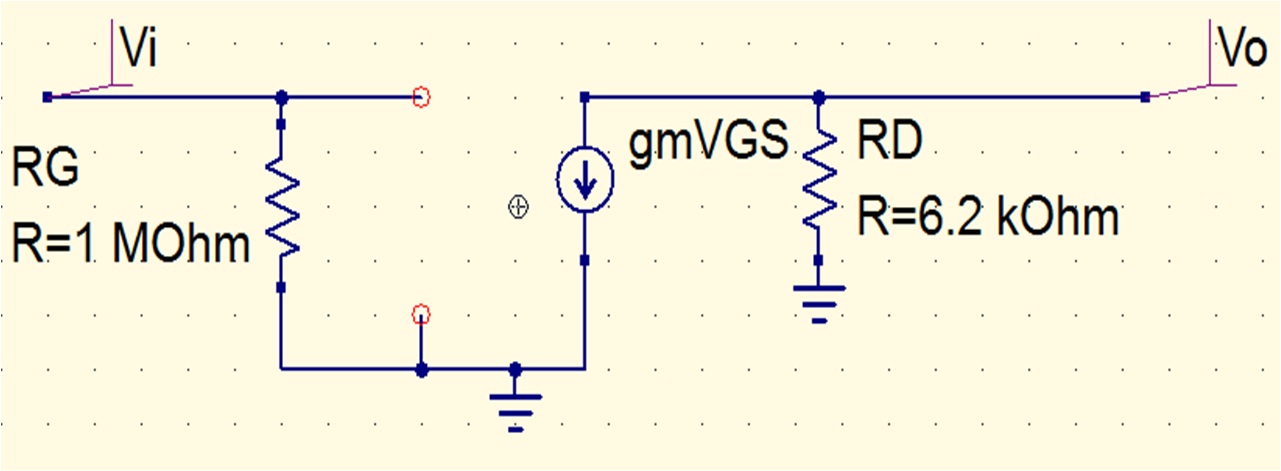
\includegraphics[width=15cm\textwidth]{dinamico.png}
        \caption{Modelo de circuito amplificador \ref{fig:amp} para pequeña señal con JFET}
        \label{fig:din}
    \end{figure}

    Sabiendo que la ganancia de tensión es

    \begin{equation} \label{eqgan}
        A_V = \frac{V_o}{V_i}
    \end{equation}

    donde

    \begin{equation*}
        \begin{split}
            V_o & = -g_mV_{GS}R_D \\
            V_i & = V_{GS}
        \end{split}
    \end{equation*}

    Sustituyendo en \eqref{eqgan} se tiene

    \begin{equation} \label{eqganp}
        A_V = \frac{-g_mV_{GS}R_D}{V_{GS}} = -g_mR_D
    \end{equation}

    Implementando la ecuación \eqref{eqdgm} deducida en el marco teórico

    $$g_m = -\frac{2}{V_P}\sqrt{I_DI_{DSS}}$$

    Al trabajar alrededor del punto estático de operacion

    $$g_m = -\frac{2}{-1V}\sqrt{(0.533mA)(15mA)} = 5.655 m\mho$$

    Quedando así la ganancia en \eqref{eqganp}

    \begin{equation} \label{eqAvt}
        A_V = -g_mR_D = -(5.655 m\mho)(6.2 k\Omega) = -35 V/V
    \end{equation}

    De la figura \ref{fig:din} se establece que

    \begin{equation*}
        \begin{split}
            A_V & = 35 V/V \\
            Z_i & = R_G = 1M\Omega \\
            Z_i & = R_D = 6.2k\Omega
        \end{split}
    \end{equation*}

    \newpage

    \section{Materiales e Instrumentos}

    \begin{table}[h!]
        \centering
        \caption{Equipos o instrumentos}
        \label{tab:instrumentos}
        \begin{tabular}{|c|c|c|} \hline
            Equipo                    &  Marca&    Modelo   \\ \hline
            Osciloscopio              &  UNI-T & UTD2102CEX+ \\
            Generador de Onda & UNI-T & UTG932E \\
            Fuente de alimentacion DC  &  UNI-T & UTP3305-II  \\ \hline
        \end{tabular}
    \end{table}

    \begin{table}[h!]
        \centering
        \caption{Componentes y materiales}
        \label{tab:componentes}
        \begin{tabular}{|c|c|c|} \hline
            Referencia&Descripción&    Especificaciones   \\ \hline
                  RD1 = 2.7k$\Omega$   & Resistencia   &          1/4 W         \\
                  RD2 = 3.6k$\Omega$   & Resistencia   &          1/4 W         \\
                  RG = 1M$\Omega$   & Resistencia &  1/4 W         \\
                  RS =  1.5k$\Omega$  &Resistencia  &         1/4 W         \\
                  Ci = Co = Cs = 10 \mu F & Capacitor & 25V \\
                  Q = 2N5555  & Tansistor JFET canal n &   \\ \hline
            \end{tabular}
            
    \end{table}

    \newpage

    \section{Presentación de Resultados}

    \begin{table}[h!]
        \centering
        \caption{Tensiones dc en los terminales del transistor}
        \label{tab:Q}
        \begin{tabular}{|c|c|c|c|c|c|} \hline
            $V_D$ [V]  &  $V_S$ [V] &  $V_G$ [V]  &  $I_D$ [A] & $V_{DS}$ [V] & zona \\ \hline
            2.8  ± 0.2  &  2.2 ± 0.2 &  0.000 ± 0.002  &  0.001460 \pm 0.000337  &  0.6 \pm 0.4  & ohmica \\ \hline
        \end{tabular}
    \end{table}

    \subsection{mediciones predeterminadas}

    \begin{figure}[h!]
        \centering
        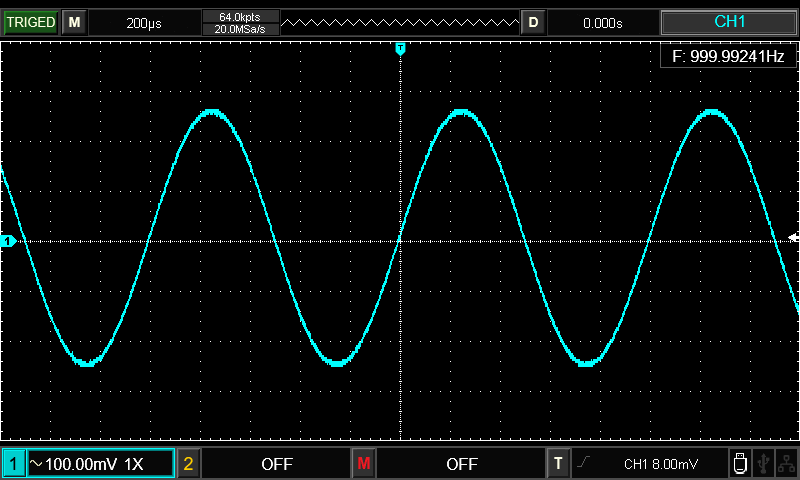
\includegraphics[height=6cm\textwidth]{p23Vi.png}
        \caption{Señal de entrada $V_i$}
        \label{fig:Vi}
    \end{figure}

    \begin{figure}[h!]
        \centering
        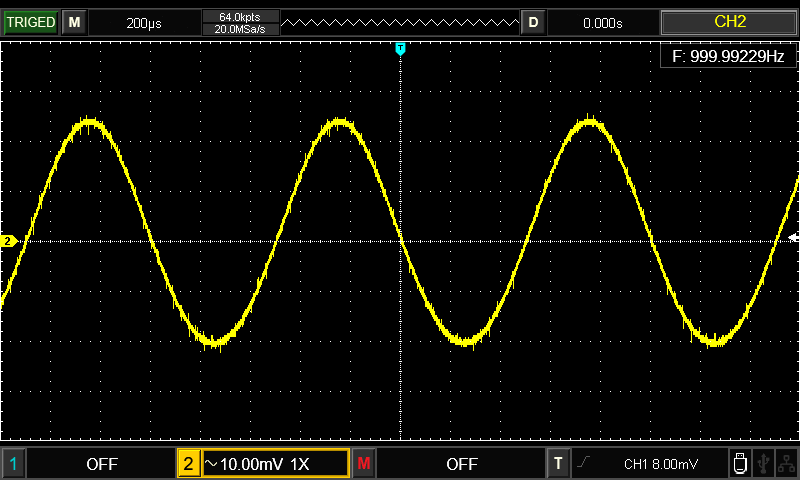
\includegraphics[height=6cm\textwidth]{p23Vo.png}
        \caption{Señal de salida $V_o$}
        \label{fig:Vo}
    \end{figure}

    \newpage

    \begin{figure}[h!]
        \centering
        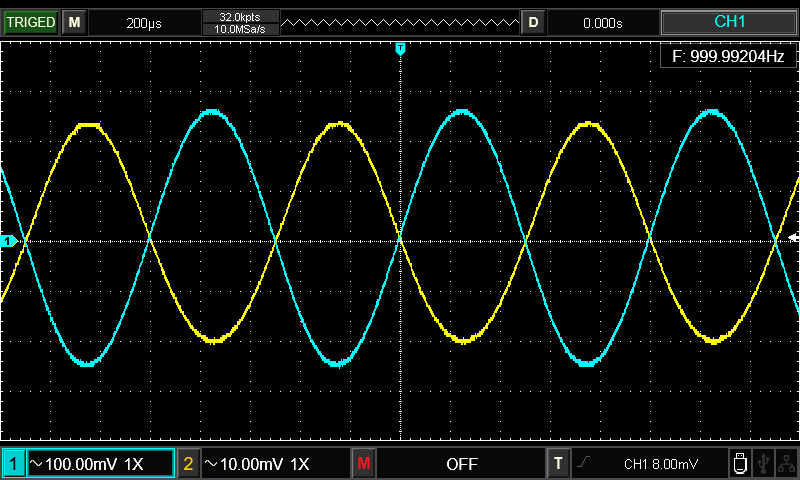
\includegraphics[height=6cm\textwidth]{p23ViVo.png}
        \caption{Señal de entrada $V_i$ (azul) y señal de salida $V_o$ (amarillo)}
        \label{fig:ViVo}
    \end{figure}

    \begin{table}[h!]
        \centering
        \caption{Descripcion de señales establecidas en la figura \ref{fig:ViVo}}
        \label{tab:p23}
        \begin{tabular}{|c|c|c|} \hline
            señal  &  tensión p-p [V] & frecuencia [Hz] \\ \hline
            $V_i$  &  520m ± 20m &  1000 ± 38  \\
            $V_o$  &  44m ± 2m &  1000 ± 38  \\ \hline
        \end{tabular}
    \end{table}

    Se calculó las ganancia de tensión experimental con la ecuacion \eqref{eqAv} referida en los anexos. Por otra parte, la ganancia teorica queda señalada en la ecuación \eqref{eqAvt} en la sección de Cálculos prévios.

    \begin{table}[h!]
        \centering
        \caption{Ganancia relacionada al amplificador de la figura \ref{fig:amp}}
        \label{tab:av}
        \begin{tabular}{|c|c|c|} \hline
            $Av_{exp} \; [V/V]$  &  $Av_{teo} \; [V/V]$  & Desviación [\%] \\ \hline
            84.62m \pm 5.04m     &       35              & 99.8   \\ \hline
        \end{tabular}
    \end{table}

    \subsection{distorsion baja de señal $V_o$}

    \begin{figure}[h!]
        \centering
        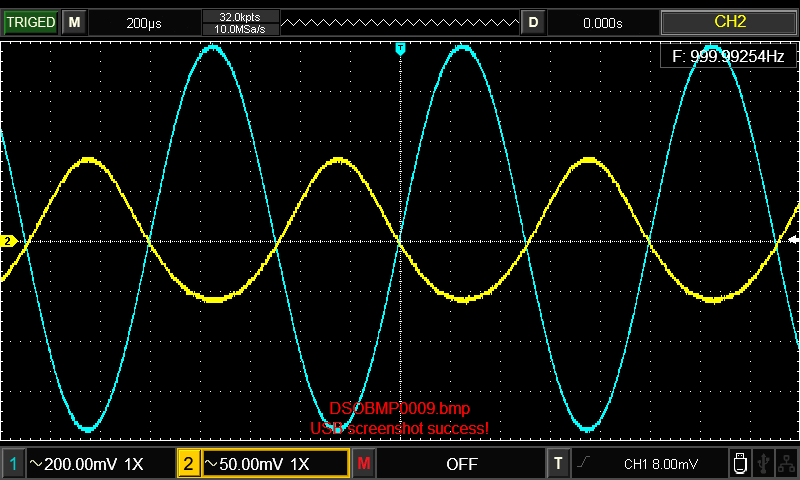
\includegraphics[height=6cm\textwidth]{p24ViVo.png}
        \caption{Leve aumento de amplitud de señal de entrada $V_o$ (azul) y su respectiva señal de salida $V_i$ (amarillo)}
        \label{fig:disViVo}
    \end{figure}

    \newpage

    \begin{figure}[h!]
        \centering
        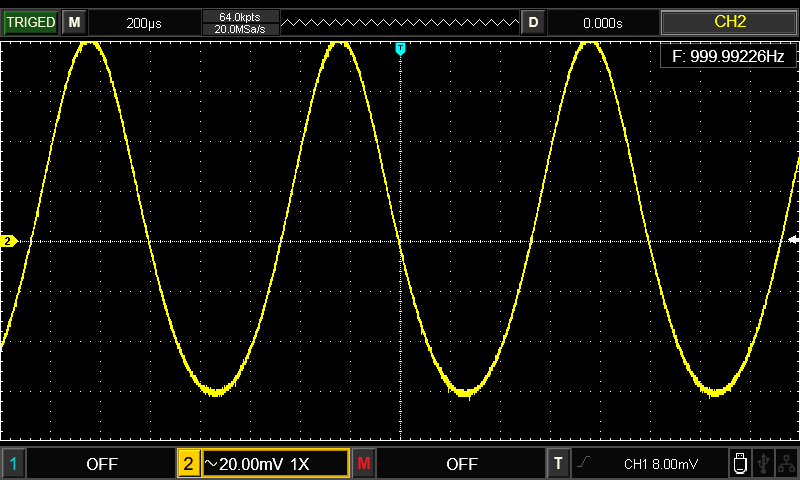
\includegraphics[height=6cm\textwidth]{p24Vo.png}
        \caption{señal de salida $V_i$ con poca distorsión}
        \label{fig:disVi}
    \end{figure}

    \begin{table}[h!]
        \centering
        \caption{Descripcion de señales establecidas en las figuras \ref{fig:disViVo} y \ref{fig:disVi}}
        \label{tab:p24}
        \begin{tabular}{|c|c|c|} \hline
            señal  &  tensión p-p [V] & frecuencia [Hz] \\ \hline
            $V_i$  &  1.52 ± 0.04 &  1000 ± 38  \\
            $V_o$  &  0.120 ± 0.004 &  1000 ± 38  \\ \hline
        \end{tabular}
    \end{table}

    \subsection{distorsion alta de señal $V_o$}

    \begin{figure}[h!]
        \centering
        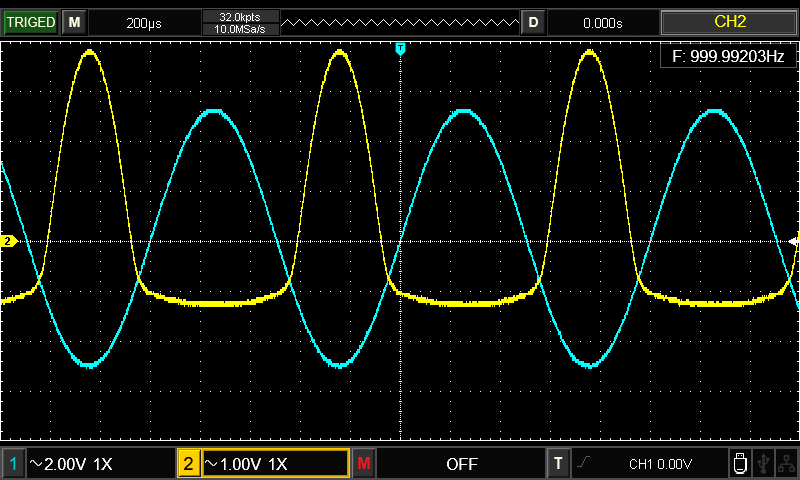
\includegraphics[height=6cm\textwidth]{p25ViVomax.png}
        \caption{Gran aumento de amplitud de señal de entrada $V_o$ (azul) y su respectiva señal de salida $V_i$ (amarillo)}
        \label{fig:disVimax}
    \end{figure}

    \newpage

    \begin{table}[h!]
        \centering
        \caption{Descripcion de señales establecidas en la figura \ref{fig:disVimax}}
        \label{tab:p25}
        \begin{tabular}{|c|c|c|} \hline
            señal  &  tensión p-p [V] & frecuencia [Hz] \\ \hline
            $V_i$  &  10.4 ± 0.4 &  1000 ± 38  \\
            $V_o$  &  5.0 ± 0.2 &  1000 ± 38  \\ \hline
        \end{tabular}
    \end{table}

    \subsection{Implementando resistencias patrón ($R_P$) para cálculo de impeancias experimentales}

    \begin{figure}[h!]
        \centering
        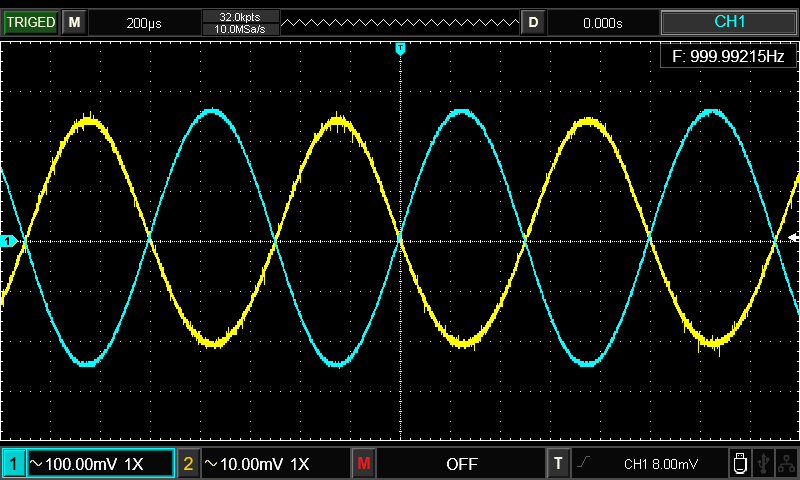
\includegraphics[height=6cm\textwidth]{p26sc.png}
        \caption{Señal de entrada $V_i$ (azul) y señal de salida $V_o$ (amarillo) sin carga}
        \label{fig:RPsc}
    \end{figure}

    \begin{figure}[h!]
        \centering
        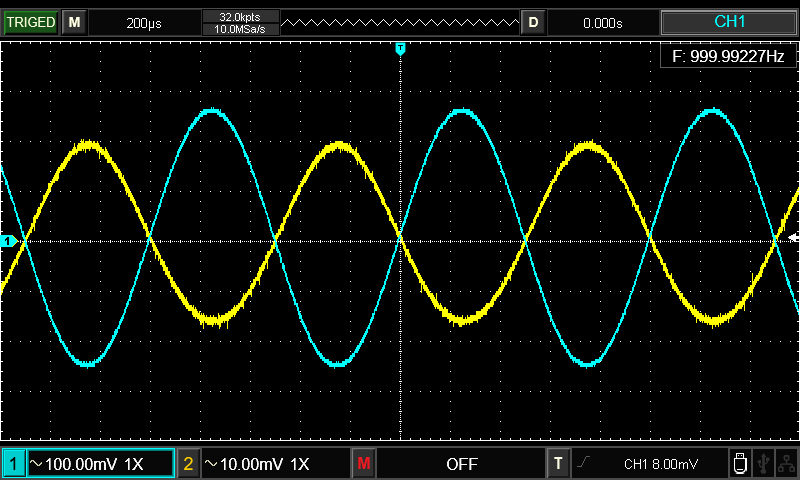
\includegraphics[height=6cm\textwidth]{p26cc.png}
        \caption{Señal de entrada $V_i$ (azul) y señal de salida $V_o$ (amarillo) con carga de $6.2k\Omega$}
        \label{fig:RPcc}
    \end{figure}

    \newpage

    \begin{figure}[h!]
        \centering
        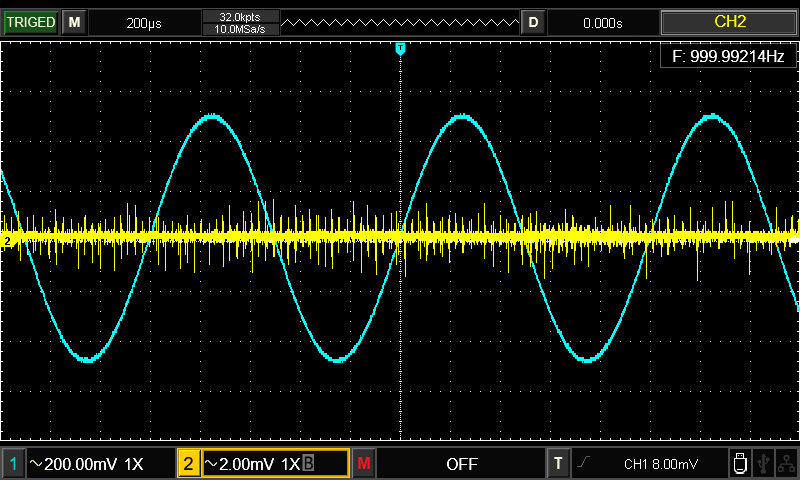
\includegraphics[height=6cm\textwidth]{p26cc1M.png}
        \caption{Señal de entrada $V_i$ (azul) y señal de salida $V_o$ (amarillo) con carga de $6.2k\Omega$ en la salida y resistencia en serie de $1M\Omega$ en la entrada}
        \label{fig:RP1M}
    \end{figure}

    \begin{table}[h!]
        \centering
        \caption{Descripcion de señales establecidas en las figuras \ref{fig:RPsc}, \ref{fig:RPcc} y \ref{fig:RP1M}}
        \label{tab:p26}
        \begin{tabular}{|c|c|c|} \hline
            señal  &  tensión p-p [V] & frecuencia [Hz] \\ \hline
            $V_i$  &  520m ± 20m &  1000 ± 38  \\
            $V_o$ sin carga  &  44m ± 2m &  1000 ± 38  \\
            $V_o$ carga $6.2k\Omega$ &  36m ± 2m &  1000 ± 38  \\
            $V_o$ carga y $R_{serie}=1M\Omega$ &  0 ± 0.002 &  1000 ± 38  \\ \hline
        \end{tabular}
    \end{table}

    \begin{table}[h!]
        \centering
        \caption{Resistencias patrones en circuito de la figura \ref{fig:amp}}
        \label{tab:rp}
        \begin{tabular}{|c|c|} \hline
            $R_{P_{Ri}}$          &  $R_{P_{Ro}}$  \\ \hline
            $1M\Omega \pm 10\%$  &  $6.2k\Omega \pm 10\%$    \\ \hline
        \end{tabular}
    \end{table}

    A partir de los valores obtenidos en las tablas \ref{tab:p26} y \ref{tab:rp}, en conjunto con las ecuaciones \eqref{eqri} y \eqref{eqro} de los anexos, se obtuvieron los siguientes valores de impedancia de entrada $R_i$ y salida $R_o$

    \newpage
    
    \begin{table}[h!]
        \centering
        \caption{Impedancia de entrada en circuito de la figura \ref{fig:circuito} con RL y CE}
        \label{tab:rpi4}
        \begin{tabular}{|c|c|c|} \hline
            $R_{i_{EXP}} [k\Omega]$  &   $R_{i_{TEO}} [k\Omega]$ & Desviación [\%]  \\ \hline
            \infty         &   1M   & \infty \\ \hline
        \end{tabular}
    \end{table}

    {\bf Observación:} debido a lo observado en la figura \ref{fig:RP1M} se considera la resistencia de entrada como un abierto en el circuito \ref{fig:amp}

    \begin{table}[h!]
        \centering
        \caption{Impedancias de salida en circuito de la figura \ref{fig:circuito} con RL y CE}
        \label{tab:rpo4}
        \begin{tabular}{|c|c|c|} \hline
            $R_{o_{EXP}} [\Omega]$  &   $R_{o_{TEO}} [\Omega]$ & Desviación [\%]  \\ \hline
            1378         &   6.2k   & 78 \\ \hline
        \end{tabular}
    \end{table}

    \begin{figure}[h!]
        \centering
        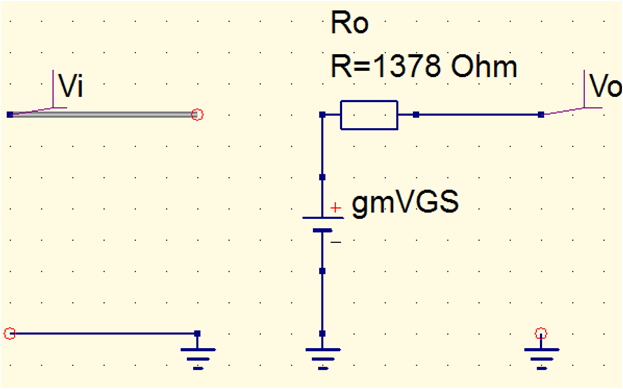
\includegraphics[height=6cm\textwidth]{modelo.png}
        \caption{Modelo lineal de amplificador del circuito de la figura \ref{fig:amp}}
        \label{fig:mod}
    \end{figure}

    \newpage

    \section{Análisis de Resultados}

    A partir de los resultados presentados se observa que el punto de operación obtenido en los cálculos prévios indica que el transistor FET está trabajando en zona de saturación, lo cual no es cierto en cuanto a la prueba de laboratorio donde debido a la tabla \ref{tab:Q} se deduce que el punto de operación está en la zona óhmica. Como consecuencia de que el transistor FET está trabajando en zona óhmica los resultados experimentales de la ganancia implican que el transistor trabaja como una resistencia y por lo tanto ocurre un proceso similar al de divisor de tensión en donde se puede observar en la figura \ref{fig:ViVo} que disminuye el voltaje pico de la salida respecto a la entrada, e incluso en algunos casos es mucho menor según la figura \ref{fig:RP1M}.

    Gracias al capacitor Cs evaluado a frecuencias media alta es posible obtener una menor impedancia de salida basándonos en el modelo hibrido y por lo tanto obtener un mejor amplificador, sin embargo, esto no es claramente visible debido a que el transistor opera en la zona óhmica como ya se mencionó.

    Basándonos en los resultados de la tabla \ref{tab:av} se observa que debido a que el transistor FET trabaja en la zona ohmica no podemos observar claramente la amplificación que produce este tipo de transistor, como tampoco se podría observar en una zona de saturación. En cambio en el BJT se pudo observar efectivamente al regular su punto de operación en la zona lineal que el transistor trabajaba como un amplificador y cumplía su función. En cuanto a las impedancias de salida y entrada en ambos circuitos, en el caso del BJT se pudo analizar que tiene una considerable ganancia de entrada en cambio en el JFET para la impedancia de entrada se establece un abierto lo cual proporciona una ventaja en cuanto a amplificación. Para las impedancias de salida, debido a la configuración se obtuvieron impedancias semejantes, siendo lo más bajas posibles pero en promedio se acercaron a 1k\Omega tanto la ganancia de BJT como el del JFET según las tablas \ref{tab:rpi4} y \ref{tab:rpo4}. 

    En cuanto a la implementación de cualquiera de los dos, es necesario considerar obtener una hoja de datos bastante razonable para el JFET lo cual es difícil de conseguir, el JFET no posee muchos modelos que tengan un voltaje de pinch off predeterminado y el IDSS que se necesita, esto puede dificultar a la hora de hacer diseños complejos, por lo que es recomendable el BJT porque existen otros modelos con otras características que se asemeja a lo que necesitamos no como el JFET que son limitados. 

    \newpage
    
    \section{Conclusiones y Recomendaciones}

    Con base a los resultados obtenidos durante la práctica se puede observar que los métodos utilizados para las mediciones y los cálculos de la ganancia, de la impedancia de entrada y la impedancia de salida son iguales a los que se utilizaron para un BJT en la practica 4. Durante la realización de esta práctica también se logró reforzar los conocimientos vistos en clase y junto con los resultados obtenidos se puede inferir que la amplificación en un circuito con el JFET depende más de las propiedades del transistor más que de los elementos de su red de polarización.

    Se pudo realizar completamente la práctica y se pudieron cumplir satisfactoriamente los objetivos planteados los cuales eran: estudiar el comportamiento dinámico de una estructura básica amplificadora JFET canal n y obtener experimentalmente las características más importantes de un amplificador como son: la ganancia de tensión, impedancia de entrada e impedancia de salida, las cuales pueden variar según el tipo de transistor y sus características.

    \newpage

    \section{Bibliografía}

    \begin{itemize}
        \item Sedra Adel. “Circuitos Microelectrónicos”. En: OXFORD University Press 4 (2002). [1]
        \item Héctor Navarro. “Clases de Transistor de Efecto de Campo”. En (2024). Documento digital. [2]
        \item Panayotis Tremante. "Método resistencia patrón". En (2024). Documento digital. [3]
        \item Gusrtavo Ruiz. "Electrónica básica para ingenieros". En: Dpto. Electrónica y Computadores, Facultad de Ciencias, Universidad de Cantabria (2001). [4]
    \end{itemize}
    
    \printbibliography

    \newpage

    \section{Anexos}

    \subsection{Cálculo del punto de operación}

    Para los valores $V_{DS}$ y $I_D$ de la \ref{tab:Q} se realizaron los siguientes cálculos:

    Sabiendo que $V_{DD} = 12 \pm 1 [V]$

    \begin{equation}
        V_{DS} = V_D - V_S
        \label{Qeq1}
    \end{equation}

    \begin{equation}
        I_D = \frac{V_{DD} - V_D}{R_D}
        \label{Qeq2}
    \end{equation}

    Para el cálculo de sus respectivas incertidumbres:

    \begin{equation}
        \Delta V_{DS} = \Delta V_D + \Delta V_S
        \label{Qeq3}
    \end{equation}

    \begin{equation}
        \begin{split}
            \Delta I_D & = \left | \frac{\partial I_D}{\partial V_{DD}} \right | \Delta V_{DD} + \left | \frac{\partial I_D}{\partial V_D} \right | \Delta V_D + \left | \frac{\partial I_D}{\partial R_D} \right | \Delta R_D \\
            & = {1 \over R_D} \Delta V_{DD} + {1 \over R_D} \Delta V_D + \frac{V_{DD}-V_D}{R_D^2} \Delta R_D
        \end{split}
        \label{Qeq4}
    \end{equation}

    \subsection{Cálculo de ganancia}

    Para la tabla \ref{tab:av} se calculó la ganancia a través de la siguiente ecuación, basandose en la ecuación \eqref{eqgan},

    \begin{equation} \label{eqAv}
        A_V = {V_o \over V_i} \pm {V_o \over V_i}\sqrt{\left( {\Delta V_o \over V_o} \right)^2 + \left( {\Delta V_i \over V_i} \right)^2}
    \end{equation}

    donde,

    $V_o :$ tensión pico-pico de entrada

    $V_i :$ tensión pico-pico de entrada

    $\Delta V_o :$ incertidumbre de la tensión pico-pico de entrada

    $\Delta V_i :$ incertidumbre de la tensión pico-pico de salida

    \subsection{Cálculo de las impedancias de entrada}

    Se indica en [3] el método de la resistencia patrón para calcular las impedancias de entrada y salida del modelo lineal de amplificador de la figura \ref{fig:rp}

    \begin{figure}
        \centering
        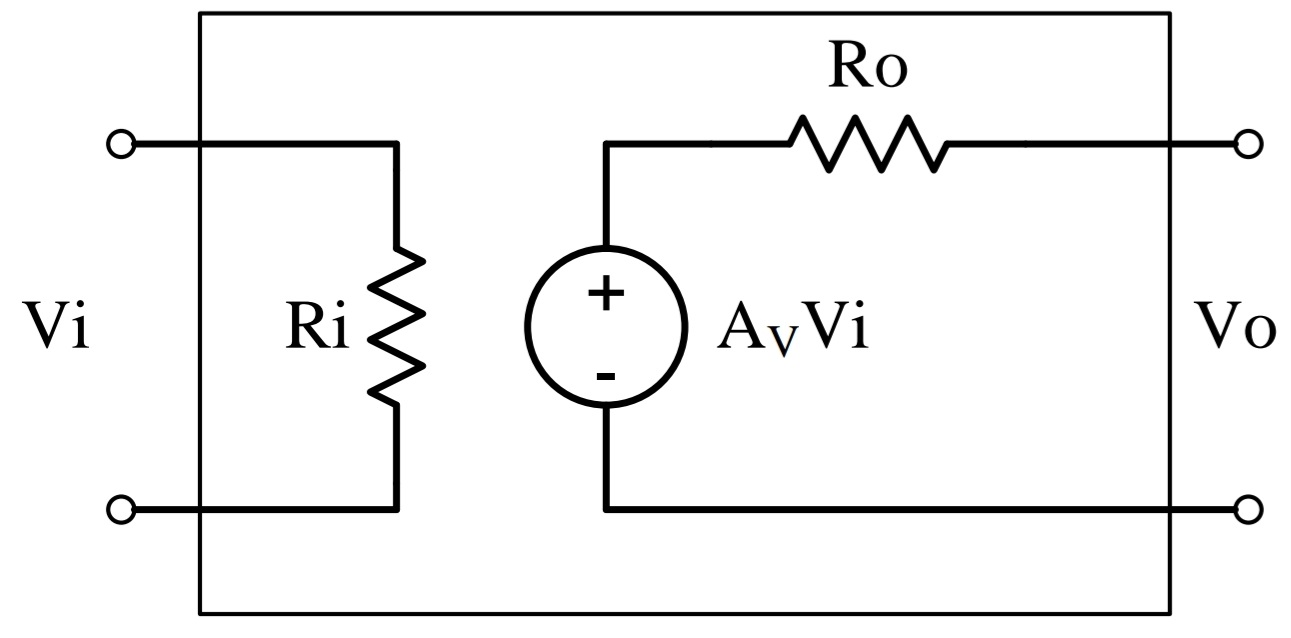
\includegraphics[height=5cm\textwidth]{zio.jpg}
        \caption{Modelo lineal de amplificador de tensión}
        \label{fig:zio}
    \end{figure}

    Para determinarlas resistencias de entrada y salida, $R_i$ y $R_o$ respectivamente, se colocan resistencias patrones $R_{PRi}$ y $R_{PRo}$ como se muestra en la Figura \ref{fig:rp} aproximadas según los valores estimados en los cálculos prévios de $R_i$ y $R_o$.

    \begin{figure}
        \centering
        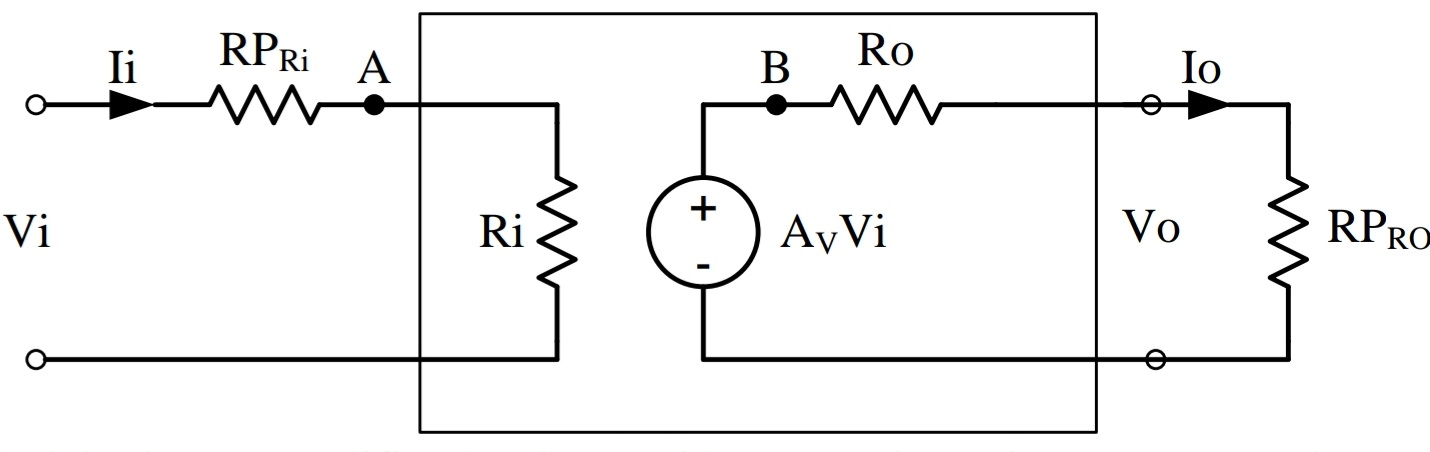
\includegraphics[height=5cm\textwidth]{RPdiagrama.jpg}
        \caption{Modelo lineal de amplificador de tensión con resistencias patrones de entrada y salida}
        \label{fig:rp}
    \end{figure}

    La corriente de entrada $I_i$ viene dada por

    $$I_i = {V_{R_{PRi}} \over R_{PRi}}$$

    También es igual a,

    $$I_i = {V_{R_{i}} \over R_{i}}$$

    Igualando ambas ecuaciones

    $${V_{R_{PRi}} \over R_{PRi}} = {V_{R_{i}} \over R_{i}}$$

    $$R_i = {V_{R_{i}} \over V_{R_{PRi}}}R_{PRi}$$

    Si $V_{R_{PRi}} = V_i - V_{R_{i}}$

    \begin{equation} \label{eqri}
        R_i = {V_{R_{i}} \over V_i - V_{R_{i}}}R_{PRi}
    \end{equation}

    Donde $V_{R_i}$ es la tensión en el punto A que se puede medir

    Para la resistencia de salida se procede de igual forma. La corriente $I_o$ viene dada por

    $$I_o = {V_{R_{PRo}} \over R_{PRo}}$$

    Por otra parte también

    $$I_o = {V_{R_o} \over R_o}$$

    Igualando ambas ecuaciones

    $${V_{R_{PRo}} \over R_{PRo}} = {V_{R_o} \over R_o}$$

    $$R_o = {V_{R_o} \over V_{R_{PRo}}}R_{PRo}$$

    $$R_o = {V_B - V_{R_{PRo}} \over V_{R_{PRo}}}R_{PRo}$$

    $V_{R_{PRo}}$ es la tension a la salida del amplificador

    $$R_o = {V_B - V_o \over V_o}R_{PRo}$$

    Al punto B de la figura \ref{fig:rp} no se tiene acceso y no se puede medir, pero esa tensión es la misma cuando el amplificador se encuentra sin carga ($V_{osc}$) y $V_o$ es la tensión con carga ($V_{occ}$), la ecuación para determinar la resistencia de salida del amplificador queda,

    \begin{equation} \label{eqro}
        R_o = {V_{osc} - V_{occ} \over V_{occ}}R_{PRo}
    \end{equation}

    \newpage

    Hojas de datos que contienen los valores experimentales recopilados en el laboratorio.

    \begin{figure}[h!]
        \centering
        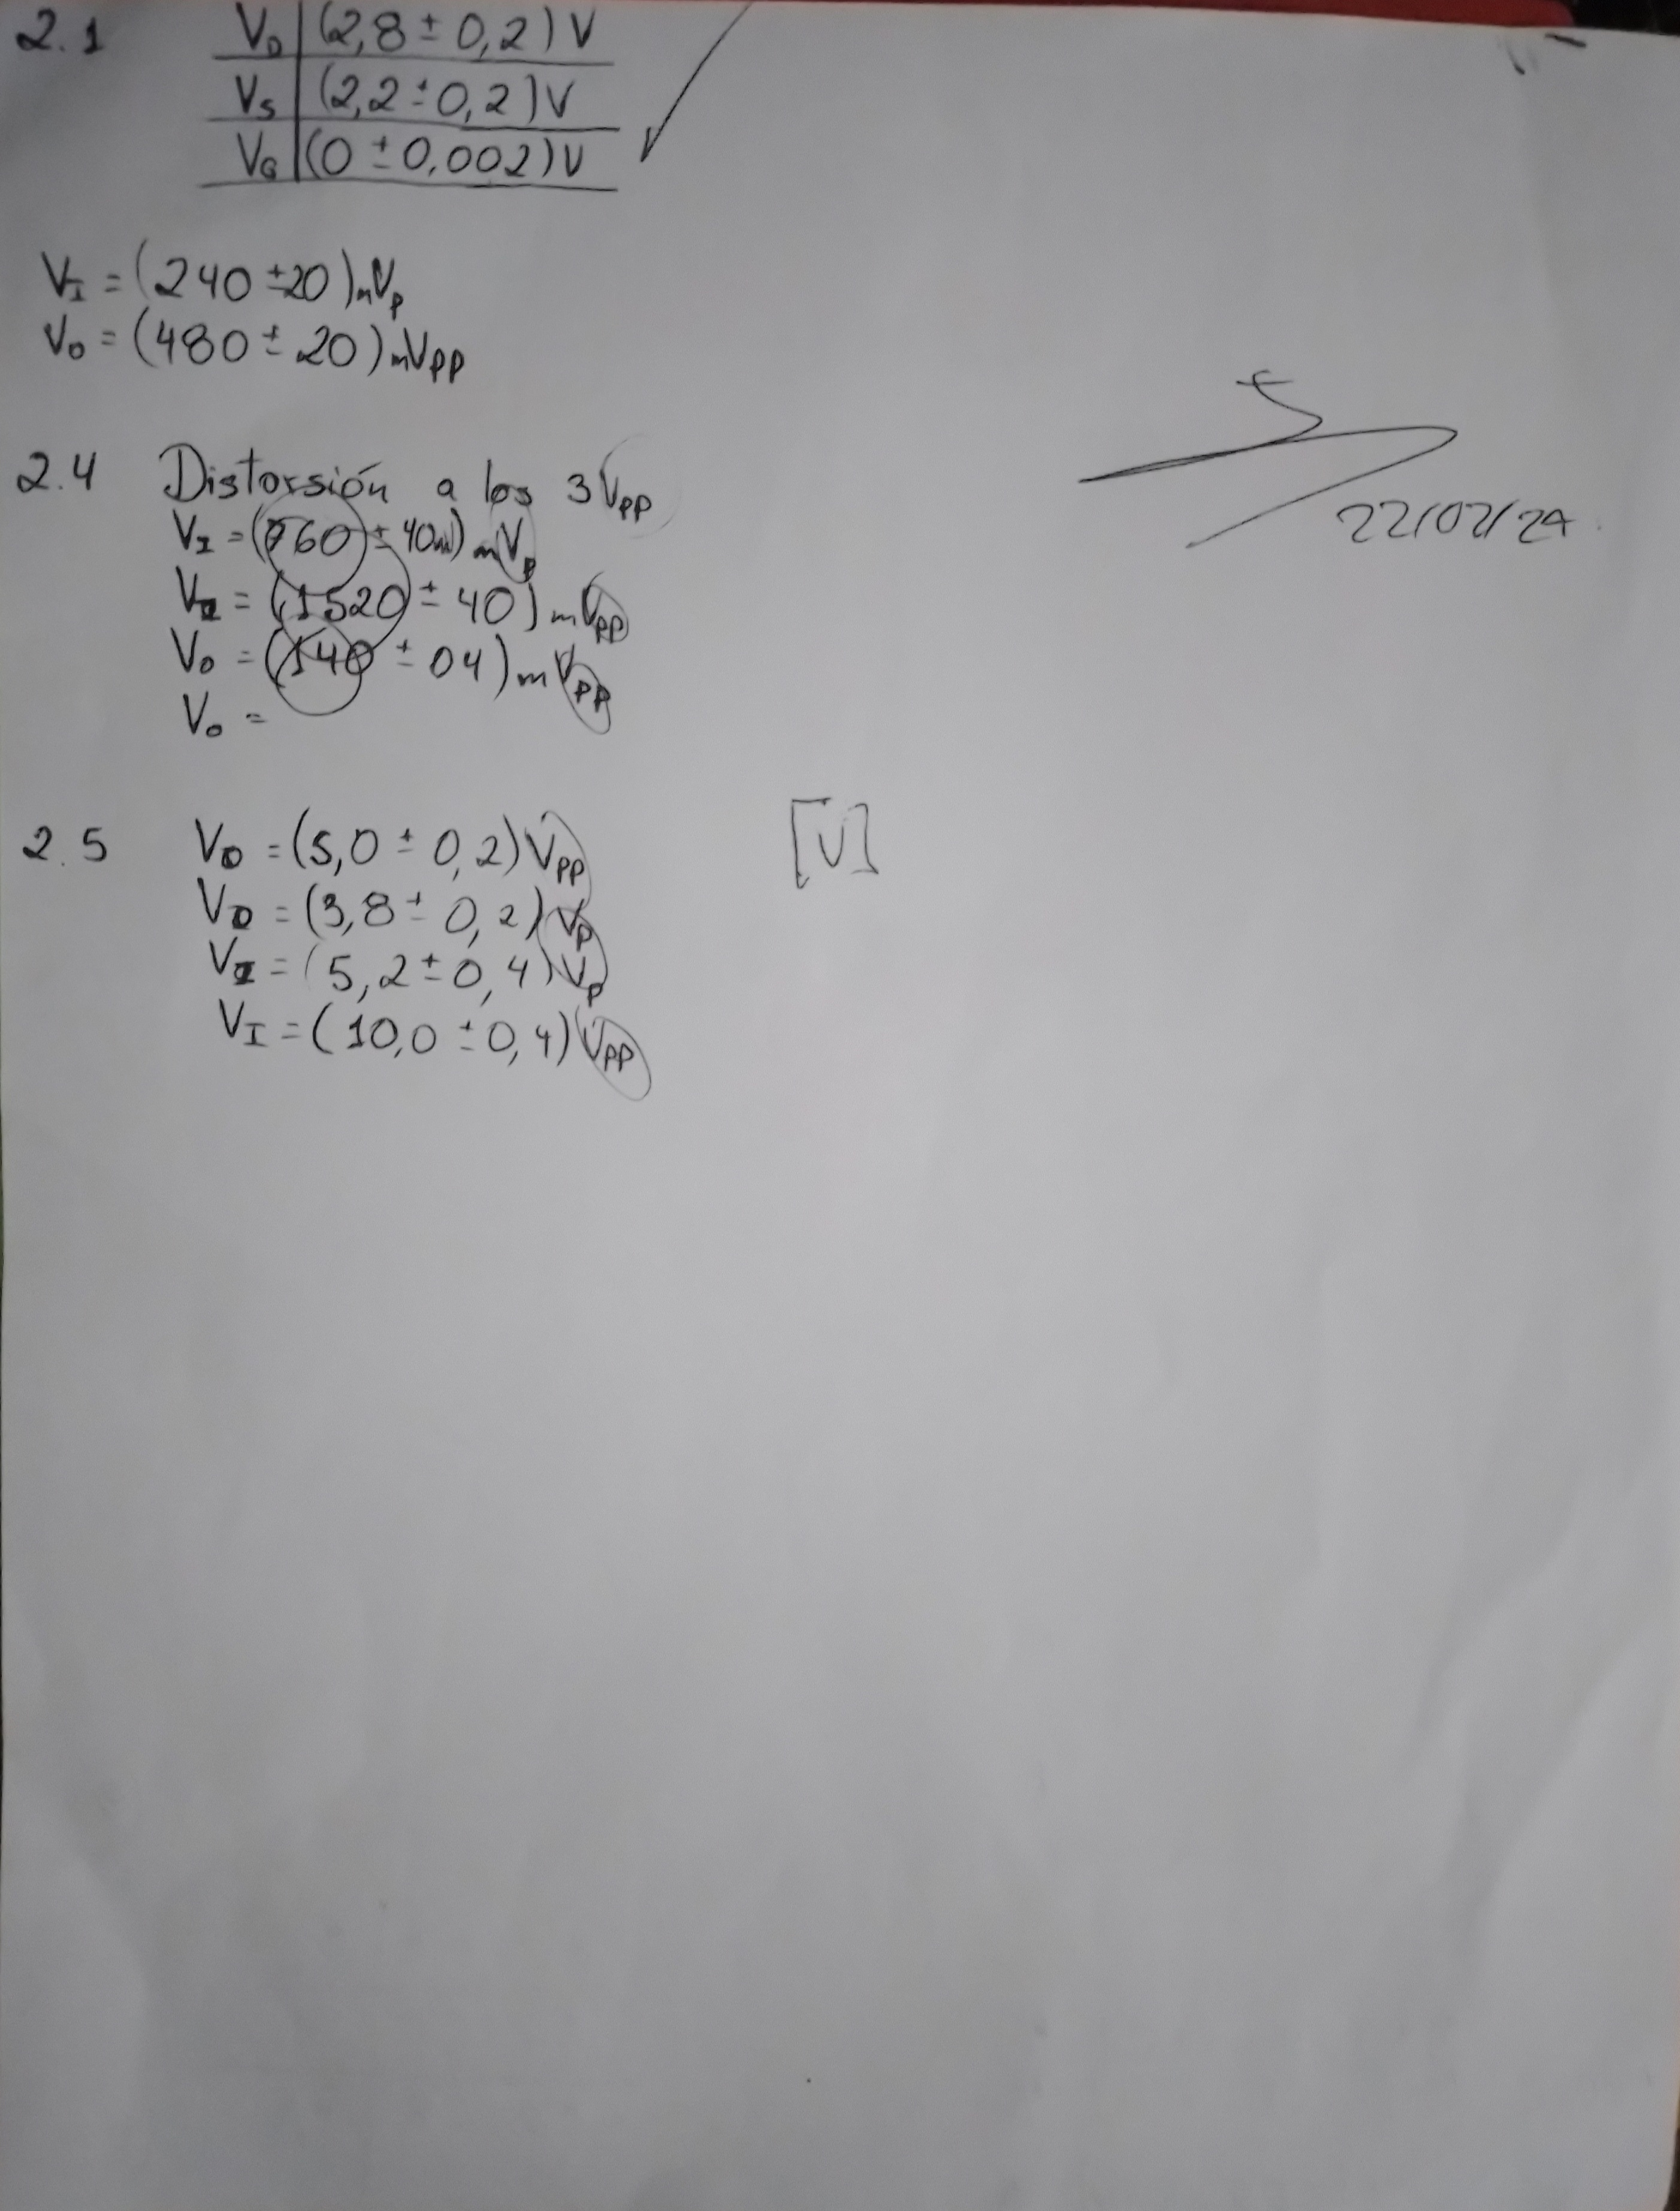
\includegraphics[height=15cm\textwidth]{hd6.jpg}
        \caption{hoja de datos}
        \label{fig:hd6}
    \end{figure}


\end{document}